\documentclass[]{article}
\usepackage{amsmath}
\usepackage{graphicx}
\usepackage{pdfpages}
\title{Physics Homework\\$\#1$}
\author{bytetriper\\\\521021910750}
\date{2022/3/2}
\begin{document}
\maketitle
\tableofcontents
\newpage
\large
\section{Regular Homework Problems}
Mainly contains Handwriten-Images\\
\begin{figure}[htbp]
    \centering
    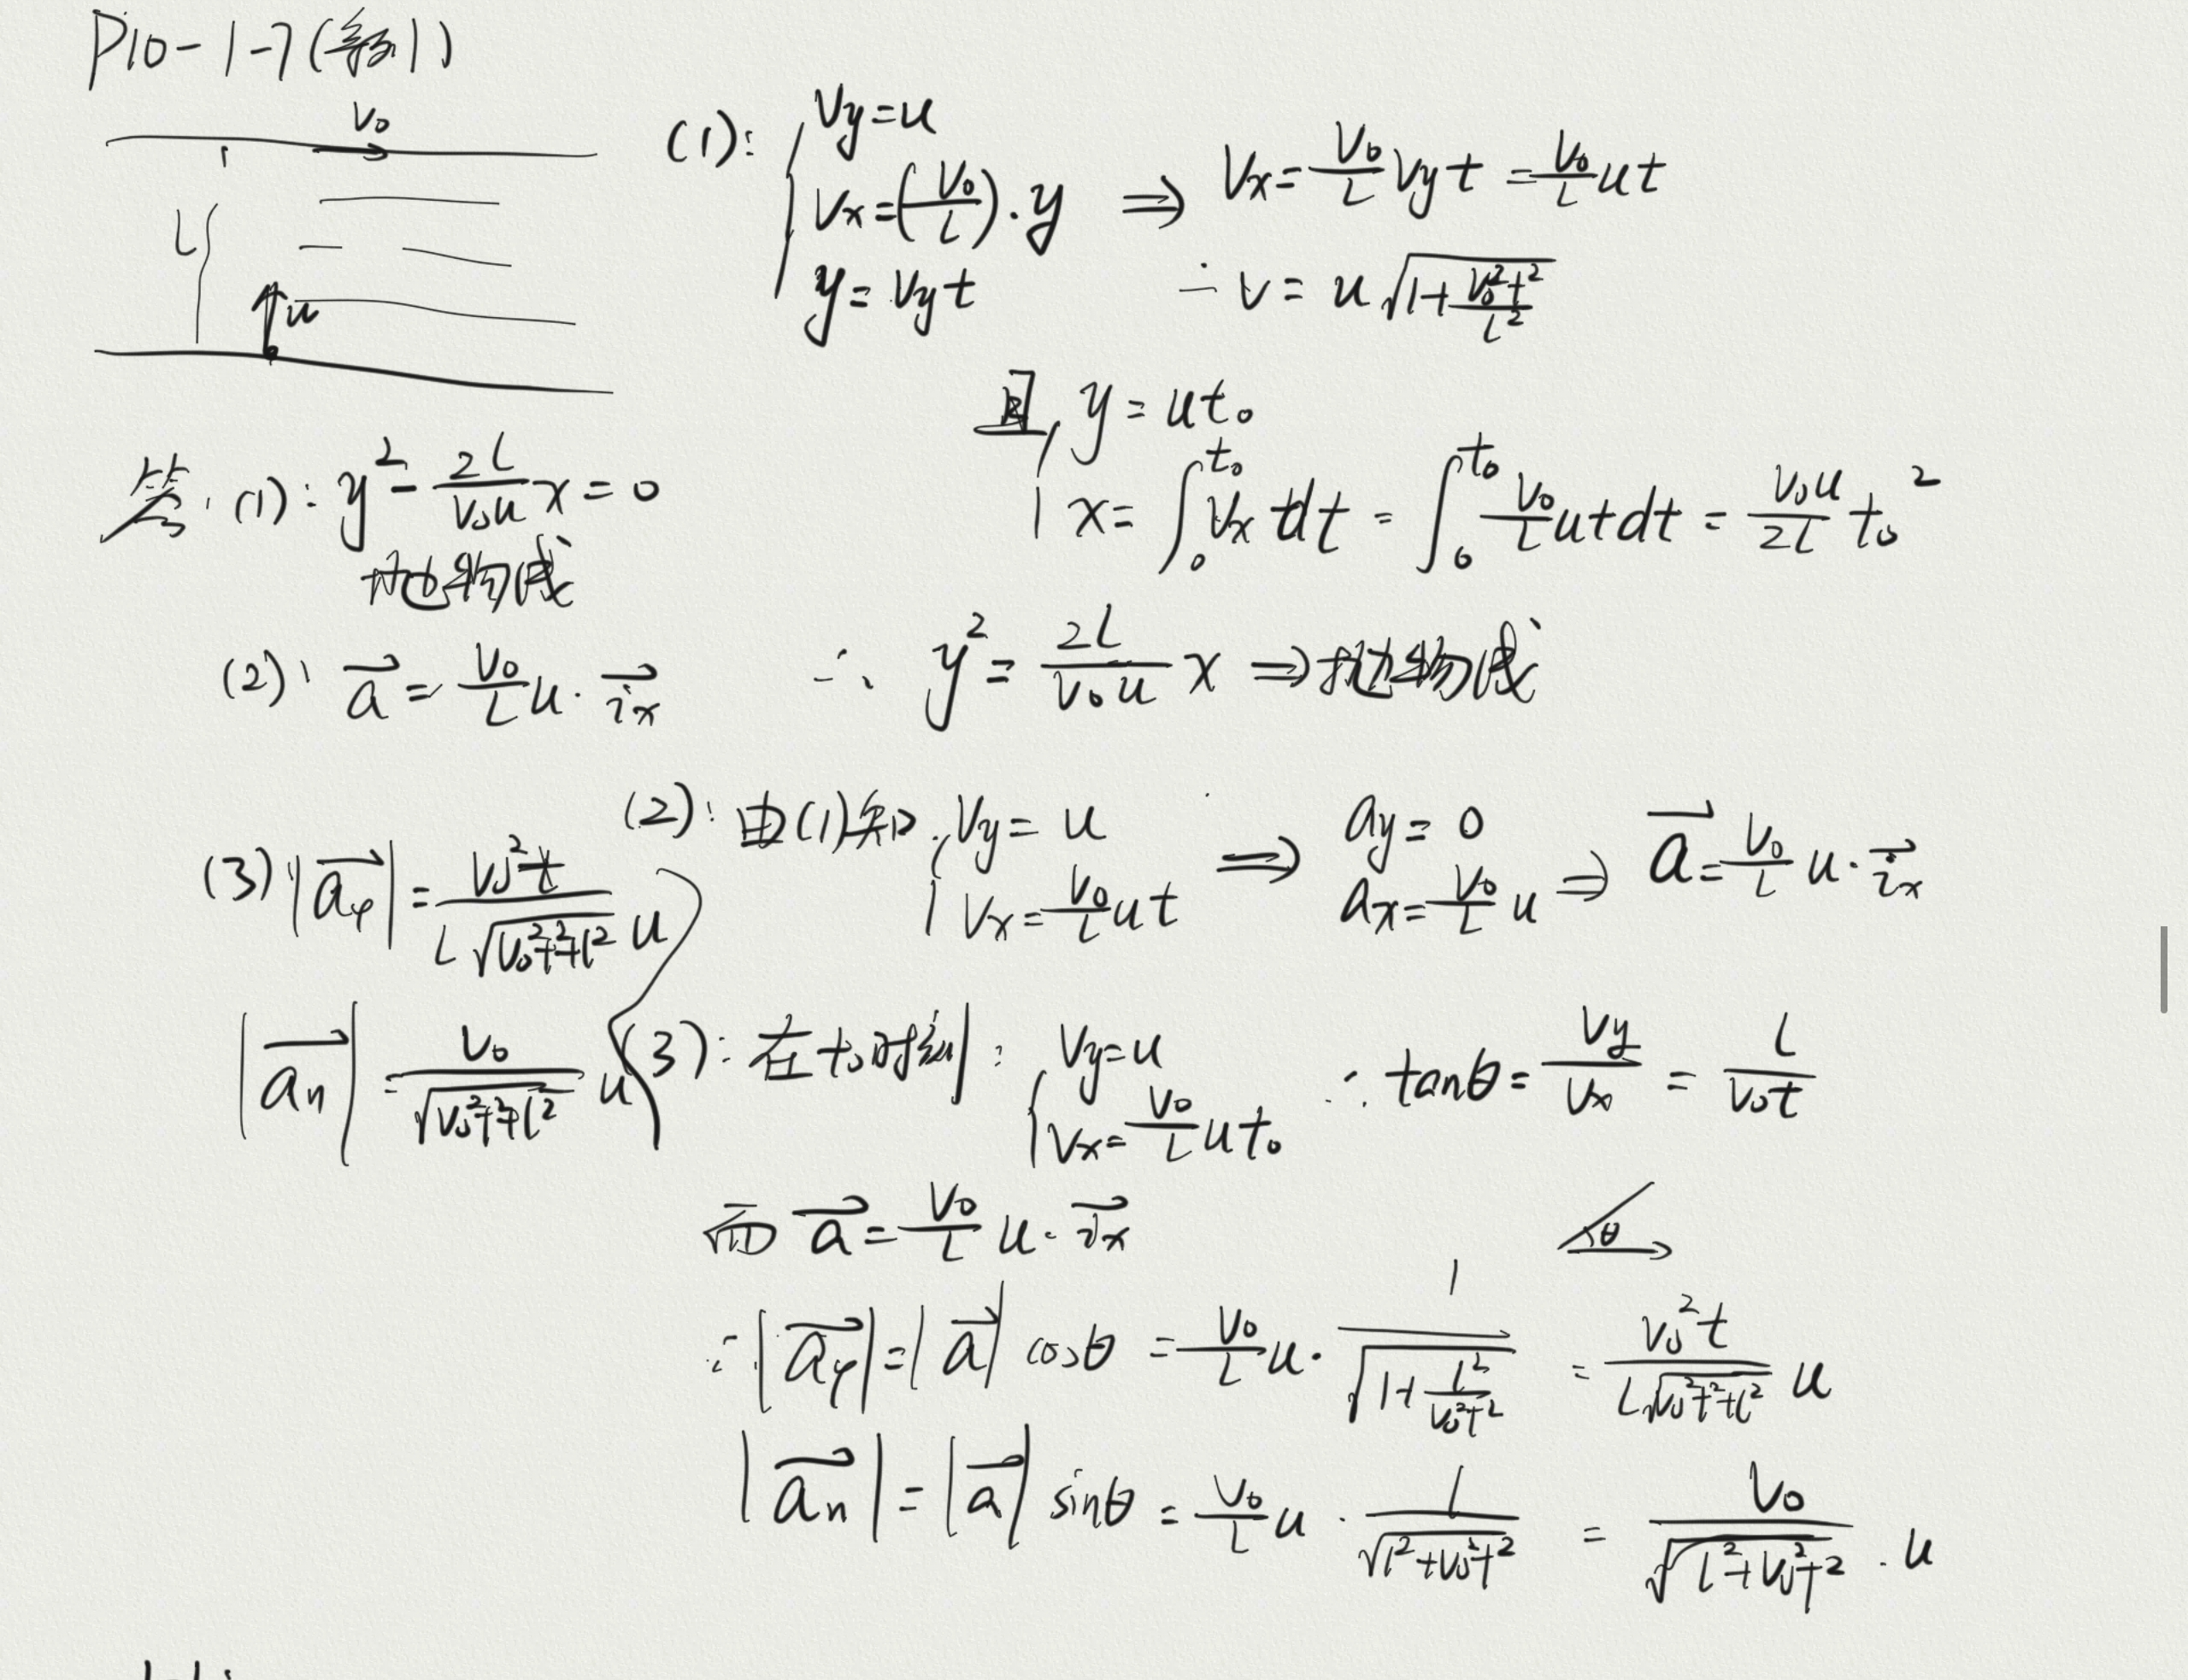
\includegraphics[width=1.3\textwidth]{1_7.jpg}
    \caption{P10-1-7}
    \label{fig:myphoto}
    \end{figure}
\begin{figure}[htbp]
    \centering
    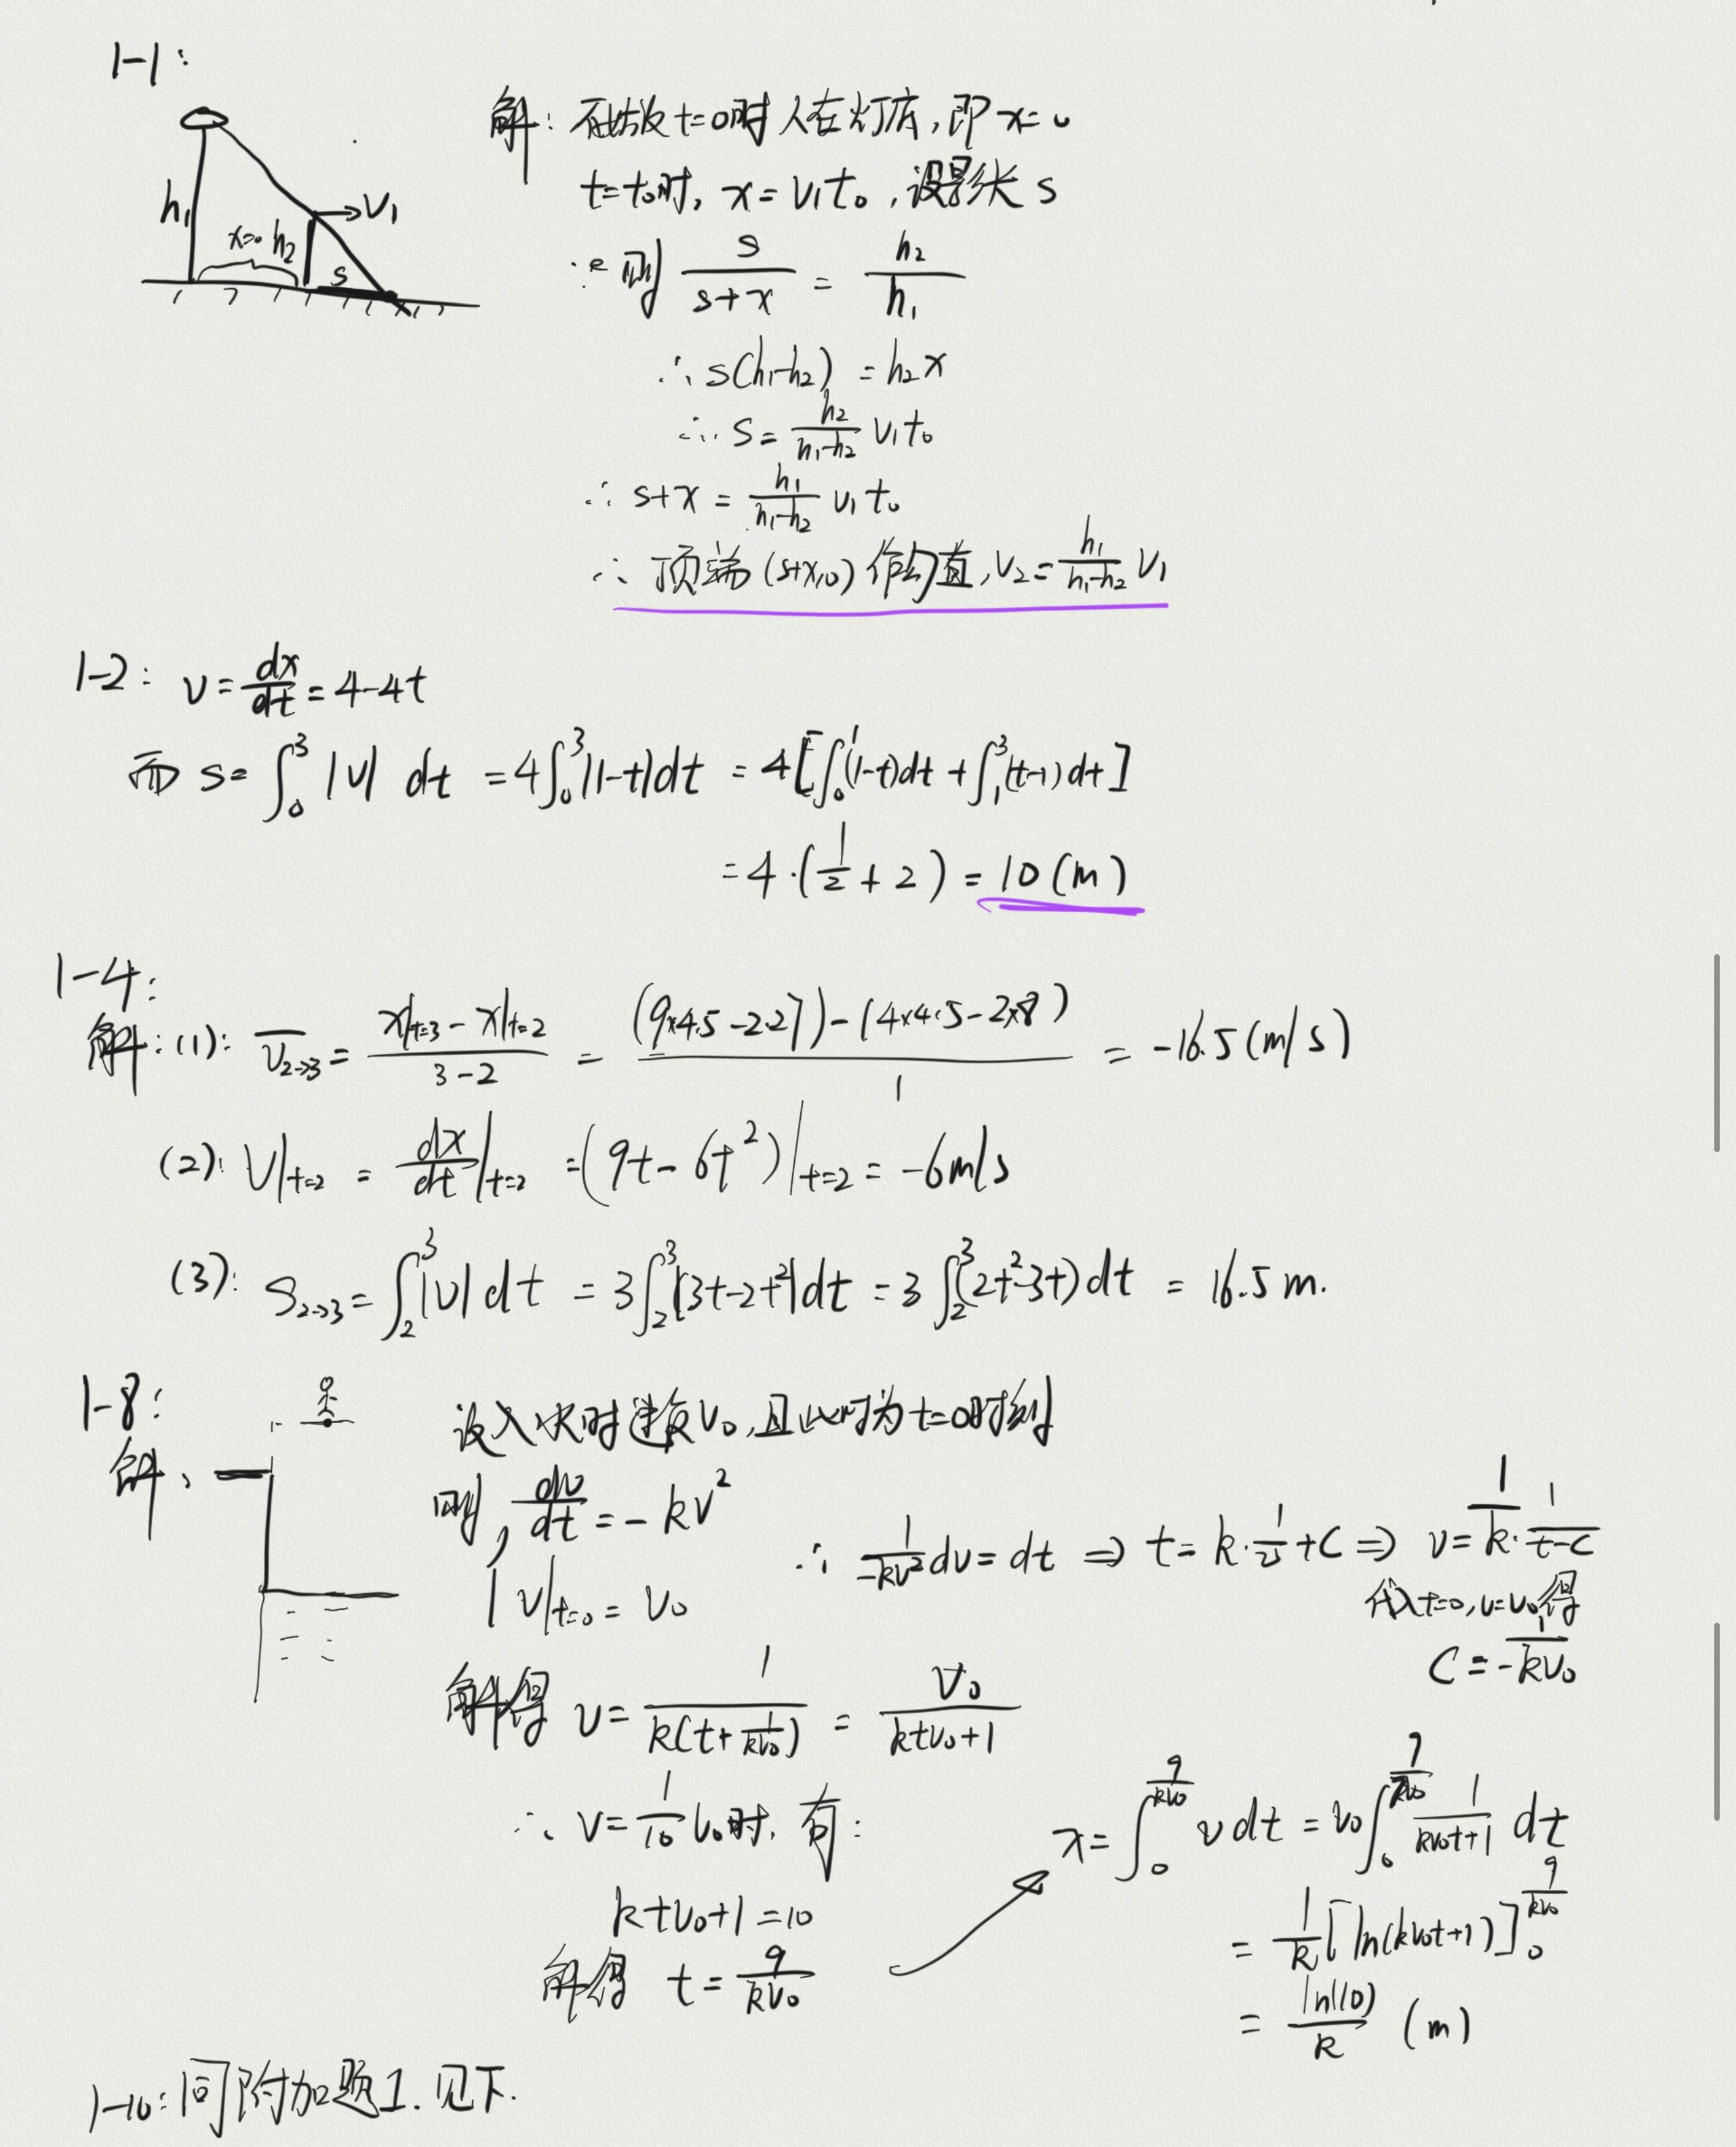
\includegraphics[width=1.2\textwidth]{1_1.jpg}
    \caption{P10:1-1 to 1-8}
    \label{fig:myphoto}
    \end{figure}
\newpage
\section{Extra Problems}
\subsection{Extra Problems}

\includepdf[pages={2,3,4}]{HW_1.pdf}
\newpage
\subsection{Computer-generated Graphs}
Using matplotlib+numpy for plots\\
\begin{figure}[htbp]
    \centering
    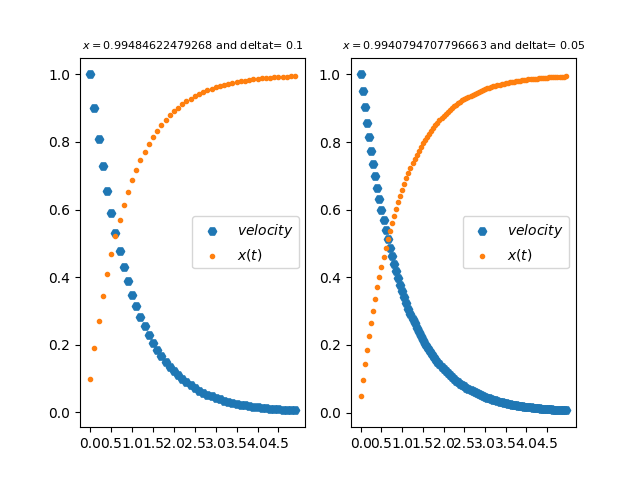
\includegraphics[width=1.5\textwidth]{Figure_1.png}
    \caption{Plot of $x(t) \& v(t)$}
    \label{fig:myphoto}
    \end{figure}
\end{document}